
In the inclusive \BtoXsgamma analysis, the aim is to reconstruct an inclusive sample of all possible \Xs states, 
as described before (e.g. \Cref{ch:exp_overview}).
This means that explicit requirements on the momentum, number of tracks, angles etc. of the \Xs system may introduce a direct bias on the `inclusiveness' of the measurement.
Assessing the impact of such selections on $X_s$ in a model-independent way is difficult.
Therefore, the \Xs system is treated in a completely `missing-momentum' approach, such that no direct requirements on it are imposed.
The reconstruction requirements are only applied on the candidate tag-$B$ meson and the candidate high-energy photons from \BtoXsgamma.
\subsection{Tag-\texorpdfstring{$B$}{B} meson candidate reconstruction}\label{sec:tag_reconstruction}

The analysis begins with a reconstruction of a tag-$B$ meson candidate in each event
using the Belle II Full Event Intepretation (\FEI) algorithm \cite{Keck:2017mui,Keck:2018lcd}, which is part of \basftwo.
It is a hierarchical six-stage reconstruction sequence, which begins with the identification of all tracks, displaced vertices (tracks that do not begin near the interaction point) and \ECL clusters.
The algorithm begins by combining track and ECL cluster information to reconstruct final-state candidate particles,
such as $\epm$, $\mupm$, $\gamma$,  $\pi^{\pm}$, $K^{\pm}$ and $K_L^0$.
In the next stage, the final-state particles are combined to form intermediate particles, such as $\piz, K_S^0, D^{(*)}$, or $B$ mesons.
In later stages, intermediate and final-state particles are combined into $B$ mesons.
At every stage of the procedure, the probability for the combined particle to be correct is evaluated by a \BDT
which maps input features related to the particle (four-momentum, vertex position, angles between daughter particles etc.) to a single classifier
output score. The final output score related to the quality of reconstruction of the $B$ meson is denoted as \feiProb. 
The schematic visualisation of the reconstruction process is shown in \Cref{fig:fei_schematic}
\begin{figure}[htbp!]
    \centering
    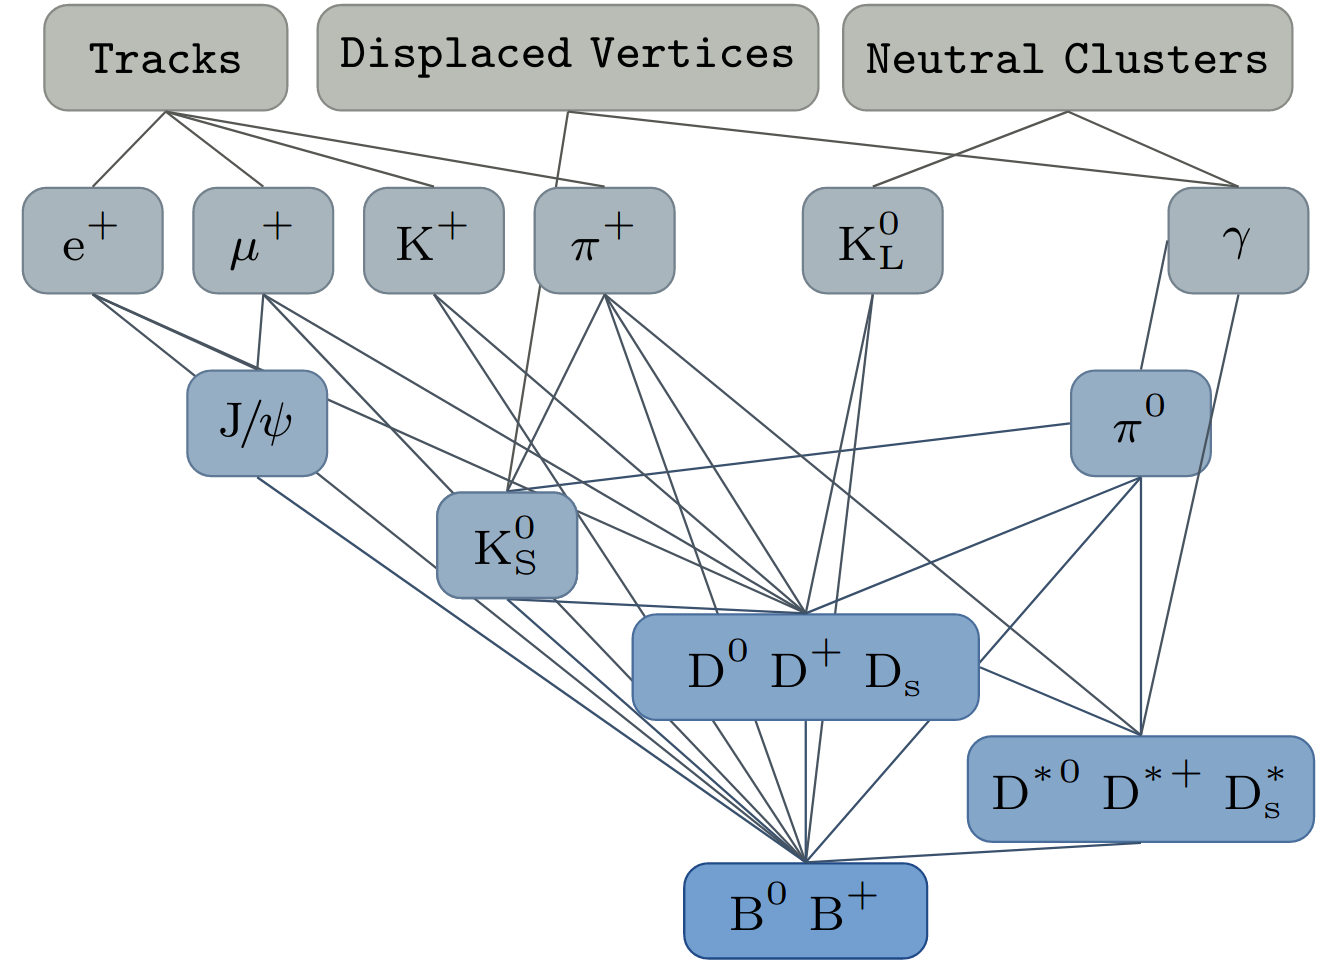
\includegraphics[width=0.45\textwidth]{figures/event_reconstruction/FEI_tagging.png}
    \caption{\label{fig:fei_schematic} 
    The schematic overview of \FEI.
    The algorithm reconstructs $B^+$ and $B^0$ candidates in 36 and 32, respectively, decay chains
    in six reconstruction stages that combine final-state and intermediate particles.
    Credit to Ref.~\cite{Keck:2018lcd}.
    }
\end{figure}

In total, \FEI reconstructs $\order(10000)$ distinct decay chains and provides $B^+$ meson candidates in 36 decay modes, and $B^0$ candidates in 32 decay modes.
As a result, two \FEI modes are differentiated: 
\feiBp, which combines \Bpm meson candidates;
and \feiBz, which combines \Bz meson candidates.
Each event may have more than one candidate reconstructed in the same and/or different decay channels and/or \FEI modes.
The reconstructed decay channels for \feiBp and \feiBz modes are shown in \Cref{tab:fei_modes}.

\begin{table}
    \centering
    \caption{\label{tab:fei_modes}
    The $B$ meson decay modes reconstructed by the \FEI algorithm.
    \FEI modes reconstructed as \feiBp and \feiBz are separated.
    }
    \begin{tabular}{|l|l|l|}
    \hline
    &\feiBp modes & \feiBz modes\\
    \hline
    1.&$B^{+} \rightarrow \bar{D}^{0} \pi^{+}$                         &     $B^{0} \rightarrow D^{-} \pi^{+}$ \\
    2.&$B^{+} \rightarrow \bar{D}^{0} \pi^{+} \pi^{0}$                 &     $B^{0} \rightarrow D^{-} \pi^{+} \pi^{0}$ \\
    3.&$B^{+} \rightarrow \bar{D}^{0} \pi^{+} \pi^{0} \pi^{0}$         &     $B^{0} \rightarrow D^{-} \pi^{+} \pi^{0} \pi^{0}$\\
    4.&$B^{+} \rightarrow \bar{D}^{0} \pi^{+} \pi^{+} \pi^{-}$         &     $B^{0} \rightarrow D^{-} \pi^{+} \pi^{+} \pi^{-}$\\
    5.&$B^{+} \rightarrow \bar{D}^{0} \pi^{+} \pi^{+} \pi^{-} \pi^{0}$  &     $B^{0} \rightarrow D^{-} \pi^{+} \pi^{+} \pi^{-} \pi^{0}$\\
    6.&$B^{+} \rightarrow \bar{D}^{0} D^{+}$                           &     $B^{0} \rightarrow \bar{D}^{0} \pi^{+} \pi^{-}$\\
    7.&$B^{+} \rightarrow \bar{D}^{0} D^{+} K_{S}^{0}$                 &     $B^{0} \rightarrow D^{-} D^{0} K^{+}$\\
    8.&$B^{+} \rightarrow \bar{D}^{0 *} D^{+} K_{S}^{0}$               &     $B^{0} \rightarrow D^{-} D^{0 *} K^{+}$\\
    9.&$B^{+} \rightarrow \bar{D}^{0} D^{+*} K_{S}^{0}$                &     $B^{0} \rightarrow D^{-*} D^{0} K^{+}$\\
    10.&$B^{+} \rightarrow \bar{D}^{0 *} D^{+*} K_{S}^{0}$              &     $B^{0} \rightarrow D^{-*} D^{0 *} K^{+}$\\
    11.&$B^{+} \rightarrow \bar{D}^{0} D^{0} K^{+}$                     &     $B^{0} \rightarrow D^{-} D^{+} K_{S}^{0}$\\
    12.&$B^{+} \rightarrow \bar{D}^{0 *} D^{0} K^{+}$                   &     $B^{0} \rightarrow D^{-*} D^{+} K_{S}^{0}$\\
    13.&$B^{+} \rightarrow \bar{D}^{0} D^{0 *} K^{+}$                   &     $B^{0} \rightarrow D^{-} D^{+*} K_{S}^{0}$\\
    14.&$B^{+} \rightarrow \bar{D}^{0 *} D^{0 *} K^{+}$                 &     $B^{0} \rightarrow D^{-*} D^{+*} K_{S}^{0}$\\
    15.&$B^{+} \rightarrow D_{s}^{+} \bar{D}^{0}$,                      &       $B^{0} \rightarrow D_{s}^{+} D^{-}$\\
    16.&$B^{+} \rightarrow \bar{D}^{0 *} \pi^{+}$                       &     $B^{0} \rightarrow D^{-*} \pi^{+}$\\
    17.&$B^{+} \rightarrow \bar{D}^{0 *} \pi^{+} \pi^{0}$               &     $B^{0} \rightarrow D^{-*} \pi^{+} \pi^{0}$\\
    18.&$B^{+} \rightarrow \bar{D}^{0 *} \pi^{+} \pi^{0} \pi^{0}$       &     $B^{0} \rightarrow D^{-*} \pi^{+} \pi^{0} \pi^{0}$\\
    19.&$B^{+} \rightarrow \bar{D}^{0 *} \pi^{+} \pi^{+} \pi^{-}$       &     $B^{0} \rightarrow D^{-*} \pi^{+} \pi^{+} \pi^{-}$\\
    20.&$B^{+} \rightarrow \bar{D}^{0 *} \pi^{+} \pi^{+} \pi^{-} \pi^{0}$&     $B^{0} \rightarrow D^{-*} \pi^{+} \pi^{+} \pi^{-} \pi^{0}$\\
    21.&$B^{+} \rightarrow D_{s}^{+*} \bar{D}^{0}$                      &     $B^{0} \rightarrow D_{s}^{+*} D^{-}$\\
    22.&$B^{+} \rightarrow D_{s}^{+} \bar{D}^{0 *}$                     &     $B^{0} \rightarrow D_{s}^{+} D^{-*}$\\
    23.&$B^{+} \rightarrow \bar{D}^{0} K^{+}$                           &     $B^{0} \rightarrow D_{s}^{+*} D^{-*}$\\
    24.&$B^{+} \rightarrow D^{-} \pi^{+} \pi^{+}$                       &     $B^{0} \rightarrow J / \psi K_{S}^{0}$\\
    25.&$B^{+} \rightarrow D^{-} \pi^{+} \pi^{+} \pi^{0}$               &      $B^{0} \rightarrow J / \psi K^{+} \pi^{-}$\\
    26.&$B^{+} \rightarrow J / \psi K^{+}$                              &    $B^{0} \rightarrow J / \psi K_{S}^{0} \pi^{+} \pi^{-}$\\
    27.&$B^{+} \rightarrow J / \psi K^{+} \pi^{+} \pi^{-}$              &     $B^{0} \rightarrow \Lambda_{c}^{-} p \pi^{+} \pi^{-}$\\
    28.&$B^{+} \rightarrow J / \psi K^{+} \pi^{0}$                      &     $B^{0} \rightarrow \bar{D}^{0} p \bar{p}$\\
    29.&$B^{+} \rightarrow J / \psi K_{S}^{0} \pi^{+}$                  &     $B^{0} \rightarrow D^{-} p \bar{p} \pi^{+}$\\
    30.&$B^{+} \rightarrow \Lambda_{c}^{-} p \pi^{+} \pi^{0}$           &     $B^{0} \rightarrow D^{-*} p \bar{p} \pi^{+}$\\
    31.&$B^{+} \rightarrow \Lambda_{c}^{-} p \pi^{+} \pi^{-} \pi^{+}$   &     $B^{0} \rightarrow \bar{D}^{0} p \bar{p} \pi^{+} \pi^{-}$\\
    32.&$B^{+} \rightarrow \bar{D}^{0} p \bar{p} \pi^{+}$               &     $B^{0} \rightarrow \bar{D}^{0 *} p \bar{p} \pi^{+} \pi^{-}$\\
    33.&$B^{+} \rightarrow \bar{D}^{0 *} p \bar{p} \pi^{+}$             &     \\
    34.&$B^{+} \rightarrow D^{+} p \bar{p} \pi^{+} \pi^{-}$             & \\
    35.&$B^{+} \rightarrow D^{+*} p \bar{p} \pi^{+} \pi^{-}$            & \\ 
    36.& $B^{+} \rightarrow \Lambda_{c}^{-} p \pi^{+}$                   & \\
    \hline
\end{tabular}
\end{table}


This thesis uses data and simulation samples following the standard Belle II approach, where sub-samples of data and \MC with FEI algorithm applied are produced centrally, referred to as \textit{\FEI skims}.
In order to make the \FEI algorithm more computationally efficient, event selections are made which reject events highly incompatible with one of the $B$ mesons decaying hadronically.
This decision is based on tracks and clusters as per standard Belle II reconstruction guidelines with additional selections, summarised in \Cref{tab:fei_objects}.
In essence, they ensure that only energetic tracks originating from the interaction point are selected.
They also minimise the impact of beam background clusters or clusters where no track information can be associated (outside of \CDC acceptance).

\begin{table}[htbp!]
    \centering
     \caption{\label{tab:fei_objects} Definitions for objects used in \FEI selections.}
     \resizebox{0.75\textwidth}{!}{
     \begin{tabular}{|l|c|c|} 
        \hline

     Selection description & Selection\\
     \hline
     Cleaned tracks & $  |d_0|<0.5~\cm,\quad z_0<2~\cm,\quad p_T>0.1~\gev $\\
     Cleaned \ECL clusters & $17~\degrees<\theta<150~\degrees,\quad E>0.1~\gev$\\
     \hline

     \end{tabular}
     }
\end{table}

Using the definitions of cleaned tracks and \ECL clusters, a requirement on each event is imposed, and only the events that pass these requirements are analysed by the \FEI algorithm.
The requirements are summarised in \Cref{tab:fei_precuts}.

\begin{table}[htbp!]
    \centering
     \caption{\label{tab:fei_precuts} Selections before running the \FEI algorithm.
     Cleaned tracks and clusters are defined in \Cref{tab:fei_objects}.
     }
     \resizebox{0.75\textwidth}{!}{
     \begin{tabular}{|l|c|} 
    \hline
     Selection description & Selection\\
     \hline
     Number of cleaned tracks in event \quad & $\geq 3$\\
     Number of cleaned \ECL clusters in event \quad & $\geq 3$\\
     Total measured centre-of-mass energy in the event \quad & $> 4~\gev$\\
     Total energy of cleaned \ECL clusters \quad &\multirow{2}{*}{$2~\gev<E<7~\gev$}\\
     and deposits associated with cleaned tracks \quad & \\
     \hline
    \end{tabular}
     }
\end{table}
The requirement to have at least 3 clean tracks in the event and at least 3 clean \ECL clusters is based on the fact, that a hadronic decay produces many charged tracks and photons.
Furthermore, the measured energy in the event in the \epem collision centre-of-mass frame is required to exceed 4~\gev.
This is a purely pragmatic requirement: based on the fact that no neutrinos or missing-momentum are present in a hadronic decay, the energy cannot be much lower than 5.28~\gev.
Finally, the total deposited energy registered by the \ECL in the event is required to lay between 2 and 7~\gev.
Hadronic events are expected to deposit significantly more energy than 2~\gev.
On the other hand, many lower-energetic particles should be stopped within \PXD, \SVD, \CDC or \TOP, meaning that their energy deposit in the \ECL would be negligible.
Therefore, a 7~\gev \ECL energy upper limit ensures that low-multiplicity events, such as \epem\ra\epem, are removed early for a better-optimised workflow.

The events that pass through requirements of \Cref{tab:fei_precuts} are analysed by the \FEI algorithm.
In each event, multiple \FEI candidates can be reconstructed (see \Cref{fig:fei_tag_reco_candidates}).
To focus only on the candidates that have been correctly reconstructed, selections on \DeltaE and \Mbc are made, as well as a loose requirement on \feiProb.
The selections shown in \Cref{tab:fei_skim_cuts} are standard selections that are applied on the Belle II \FEI skims.

\begin{table}[htbp!]
    \centering
     \caption{\label{tab:fei_skim_cuts} 
     Additional selections that reduce the datasets after applying \FEI, focusing only on well-reconstructed tag-side candidates.
     These \FEI skim selections are the nominal ones, which are applied on all \FEI skimmed data sets in Belle II.
     In this analysis, only the selection on the tag-\B meson is tightened in order to remove the edge effects.
     Such effects arise after applying a kinematic fit on the tag-side products.
     }
     \resizebox{0.75\textwidth}{!}{
        \begin{tabular}{|l|c|c|}
        \hline
        Variable &    \FEI skim selections  & Selections in this analysis \\
        \hline
        $\Mbc (\mathrm{tag})$ & $>5.24~\gev$ & $>5.245~\gev$  \\
        $\Delta E (\mathrm{tag})$ & \multicolumn{2}{c|}{$-0.15$ to $0.1$~\gev} \\
        \feiProb E & \multicolumn{2}{c|}{$> 0.001$}\\
        
        \hline
        
\end{tabular}
    
     }
\end{table}

The tag-side candidates that pass the nominal \FEI requirements undergo a kinematic fit \cite{Belle-IIanalysissoftwareGroup:2019dlq}, 
where the particles used to reconstruct the tag-$B$ candidate are fitted with a common vertex constraint.
No requirements about the quality of the fit are made, but candidates that fail the fit are rejected.
This improves the resolution of the $B$ meson momentum for correct candidates and may shift their momentum altogether.
Therefore, to avoid edge effects, the \Mbc selection in \Cref{tab:fei_skim_cuts} is tightened.
The tag-side selections used in this analysis are not affecting the \BtoXsgamma, 
as correct tag-side candidates with 
lower \Mbc, 
higher $|\DeltaE|$ 
or lower \feiProb (compared to \Cref{tab:fei_skim_cuts}) are not expected to be common.


\subsection{Candidate photon reconstruction}\label{sec:gamma_reconstruction}

As discussed, only the photon from \BtoXsgamma can be reconstructed while ensuring a model-independent inclusive measurement.
In order to reduce the quickly growing number of background photon candidates, only events where at least one photon with $\Estar>1.2~\gev$ are considered.
The photons must also be within the CDC acceptance ($17-150~\degrees$).
These requirements are summarised in \Cref{tab:photon_requirements}.
\begin{table}[htbp!]
    \centering
     \caption{\label{tab:photon_requirements} Requirements for photons in reconstructed events.}
     \resizebox{0.75\textwidth}{!}{
     \begin{tabular}{|l|c|}
     \hline 
     Selection description & Selection\\
     \hline
     Number of photons with \Estar>1.2~\gev & $  N(\Estar>1.2~\gev)\geq1 $\\
     Polar angle of photon & $17~\degrees<\theta<150~\degrees$\\
     \hline
     \end{tabular}
     }
\end{table}

Reconstructed photon energy is boosted to the signal $B$ meson rest frame based on the Lorentz transformation in \Cref{sec:appendix_boosting_to_b_frame}.

\subsection{Overview of the selected sample}\label{sec:reconstruction_overview}

After reconstruction, based on the \MC samples, there can be up to 20 tag-$B$ candidates.
The sample is broken down to show the relative fraction of the total number of tag-side $B$ meson candidates in 
\Cref{fig:fei_tag_reco_candidates}.
About 62\% (72\%) of events for \feiBp (\feiBz) modes have only 1 tag-side candidate.
About 21\% (18\%) of events for \feiBp (\feiBz) modes have two tag-side candidates and 8\% (5\%) has 3.
The number of candidates per event reduces quickly, but faster for \Bz modes, with roughly 2\% (1\%) 
of events having more than 5 candidates for \feiBp (\feiBz).
Note that the same event can have a \Bp and \Bz candidate reconstructed.

A similar distribution for the number of signal-side photon candidates is shown in \Cref{fig:photon_reco_candidates}.
Contrary to the tag-side, the highest energy photon is the sole candidate in the event in 98\% of the cases in generic \MC.
Studies on \BtoXsgamma signal \MC with a threshold of $\EB>1.4~\gev$ show that a single high-energy photon is expected in 99.9\% of the cases.
The $\EB>1.4~\gev$ selection is chosen pragmatically to maintain a reasonable data set memory size without losing signal events.
As the number of photon candidates grows swiftly with decreasing energy, this threshold still provides access to the majority of \BtoXsgamma decay phase space.
\begin{figure}[htbp!]
    \centering
    \subcaptionbox{\label{fig:fei_tag_reco_candidates}}{
    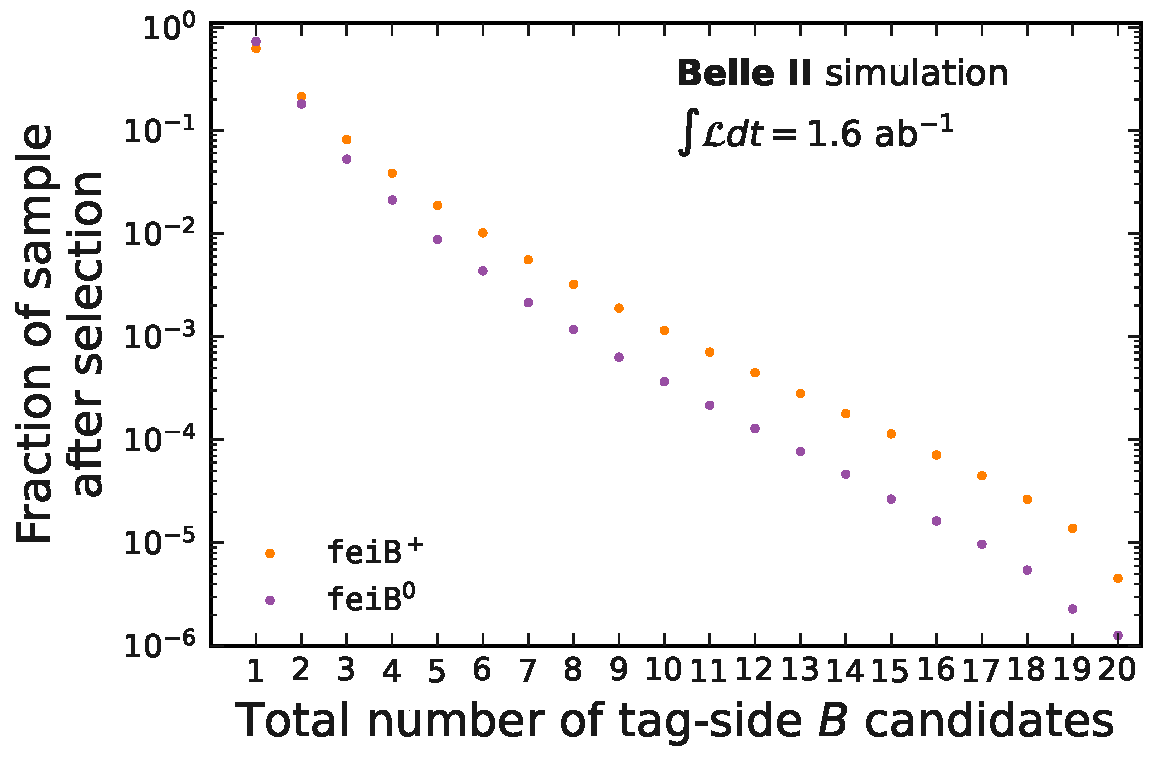
\includegraphics[width=0.45\textwidth]{figures/event_reconstruction/Bboth_total_tag_candidates.pdf}
    }
    \subcaptionbox{\label{fig:photon_reco_candidates}}{
        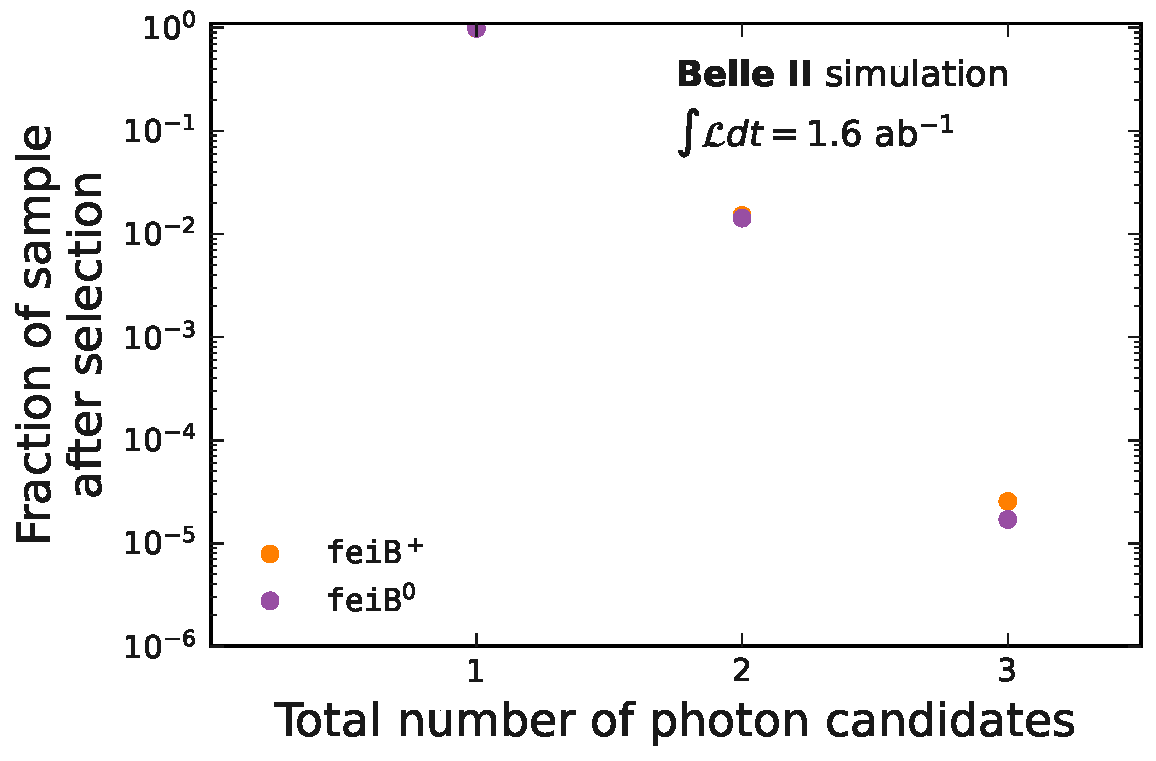
\includegraphics[width=0.45\textwidth]{figures/event_reconstruction/Bboth_total_photon_candidates.pdf}
    }
    \caption{\label{fig:reco_candidates} Relative fractions of events for the number of 
    reconstructed \B meson candidates (\Cref{fig:fei_tag_reco_candidates}) and
    reconstructed photon candidates (\Cref{fig:photon_reco_candidates}) in the generic \MC sample.
    In \Cref{fig:fei_tag_reco_candidates}, the overall volume of candidates is similar for \feiBp and \feiBz modes, 
    with around one in two events only having a single candidate per event.
    Conversely, as depicted in \Cref{fig:photon_reco_candidates},
    the vast majority of events contain only a single signal photon with $\EB>1.4~\gev$.
    Two or more photon candidates are present only $\mathcal{O}(1)\%$ of time.
    }
\end{figure}

The reconstructed \BtoXsgamma spectrum in generic \MC with the previously laid-out requirements are shown in \Cref{fig:spectrum_after_reco}.
Note that these events in general can contain multiple combinations of a photon and tag-side candidate per event.
Overall, it may seem that the \feiBz mode has a higher signal-to-background ratio compared to \feiBp.
However, one has to take into account that \feiBp and \feiBz modes result
from different reconstruction chains.
Furthermore, \feiBz has fewer modes being reconstructed than \feiBp (see \Cref{sec:tag_reconstruction}).
Therefore without additional studies that fill follow in \Cref{sec:select_tag_between_modes,sec:select_best_candidate} such a conclusion cannot be unambiguously drawn. 
On the other hand, comparing \Cref{fig:untagged_btosgamma_background,fig:spectrum_after_reco} it is clear that a better signal-to-background ratio can already be observed even without any treatment.

\begin{figure}[htbp!]
    \centering
    \subcaptionbox{\label{fig:spectrum_after_reco_bplus}}{
        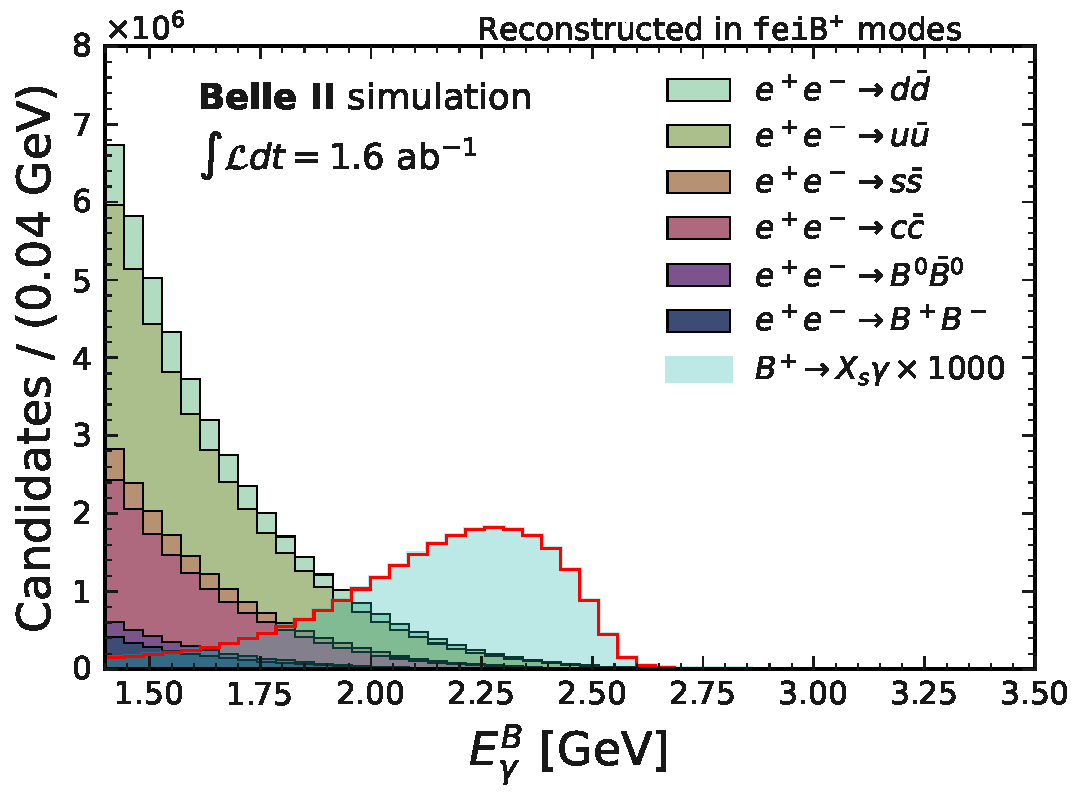
\includegraphics[width=0.45\textwidth]{figures/event_reconstruction/Bp_tagged_background.pdf}
        }
    \subcaptionbox{\label{fig:spectrum_after_reco_bzero}}{
    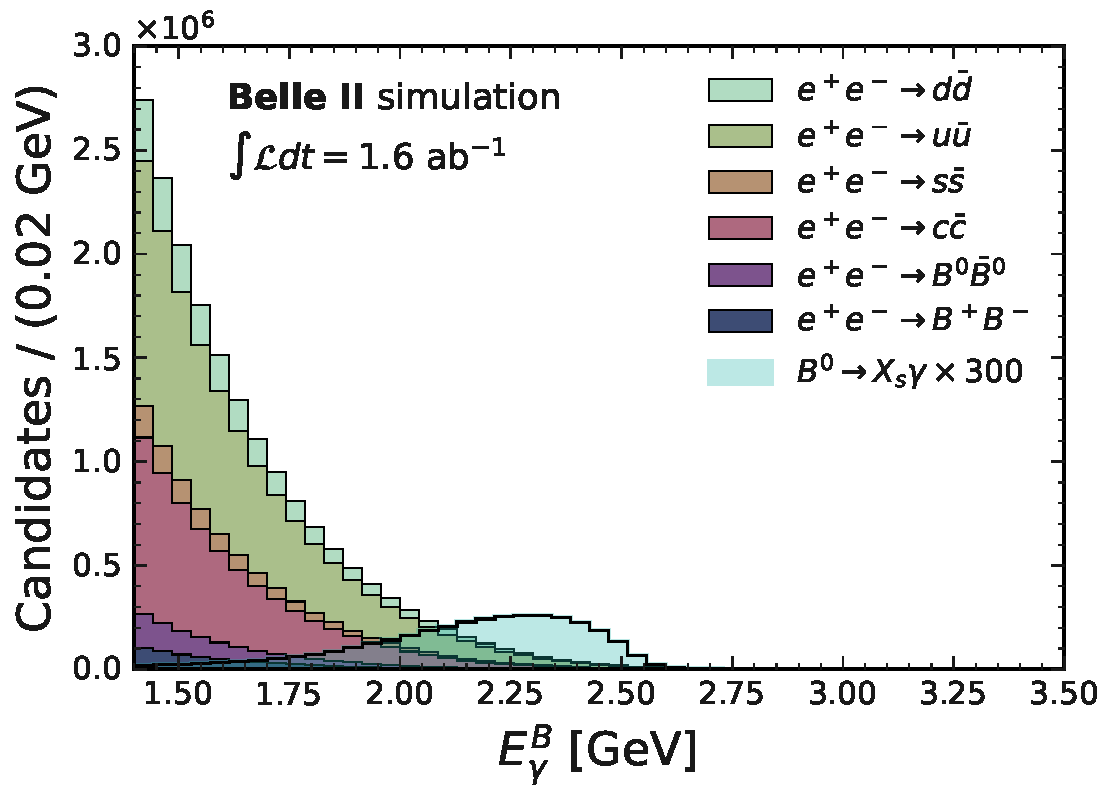
\includegraphics[width=0.45\textwidth]{figures/event_reconstruction/Bz_tagged_background.pdf}
    }
    \caption{\label{fig:spectrum_after_reco} \BtoXsgamma spectrum in generic \MC after event reconstruction in \feiBp and \feiBz modes.
    Overlaid are events from signal \MC, where the photon comes from \BtoXsgamma, multiplied by a scaling factor.
    These figures may include multiple tag-$B$ and photon entries per event and can be compared with \Cref{fig:untagged_btosgamma_background}.
    }
\end{figure}

The tag-side probability plots provided by the \FEI classifier are shown in \Cref{fig:sigprob_after_reco}.
These further emphasise the differences between tag candidates reconstructed in \feiBp and \feiBz modes.
Selecting on \feiProb variable is not trivial;
even after disregarding the differences between \feiBp and \feiBz modes, 
the \feiProb values may be different within the same-charged $B$ mode.
This is shown and discussed in \Cref{sec:appendix_fei_signal_probabilities}.
Tight direct selections, as seen in \Cref{fig:feisigprobs1,fig:feisigprobs2,fig:feisigprobs3,fig:feisigprobs4}, result in a bias for selected tag-side modes.
Therefore, no direct selections on \feiProb are applied in this analysis.

\begin{figure}[htbp!]
    \centering
    \subcaptionbox{\label{fig:sigprob_after_reco_bplus}}{
        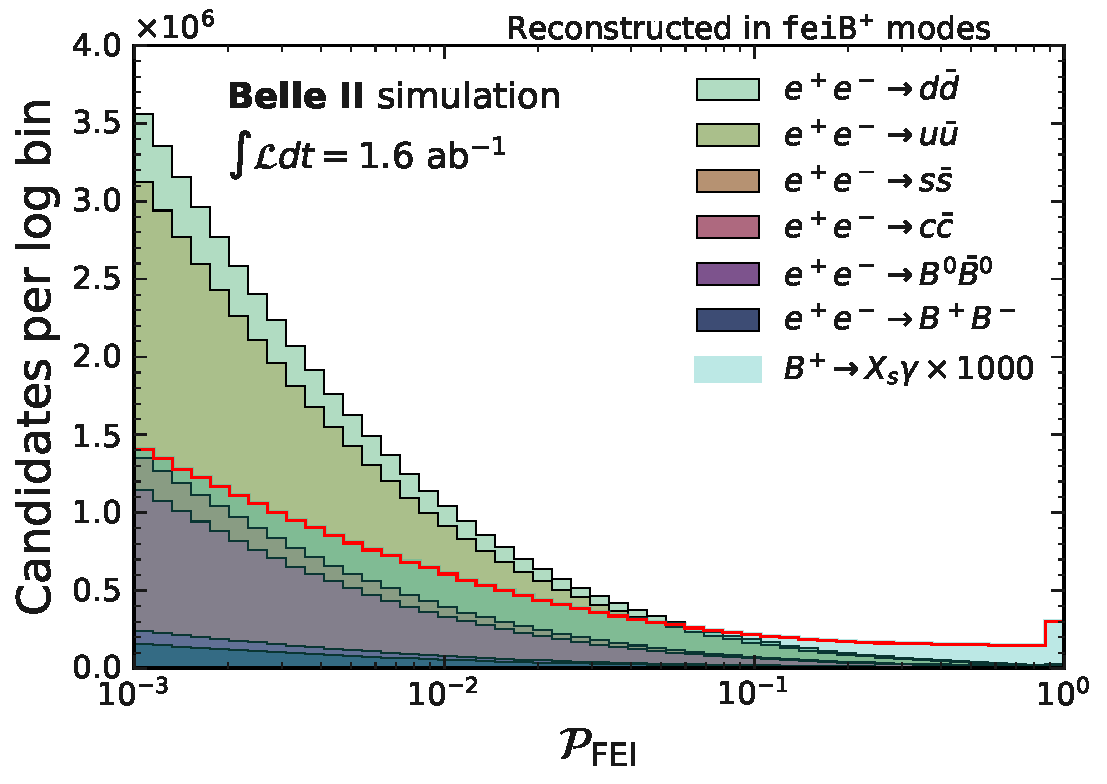
\includegraphics[width=0.45\textwidth]{figures/event_reconstruction/Bp_tagged_background_feiSigProb.pdf}
        }
    \subcaptionbox{\label{fig:sigprob_after_reco_bzero}}{
    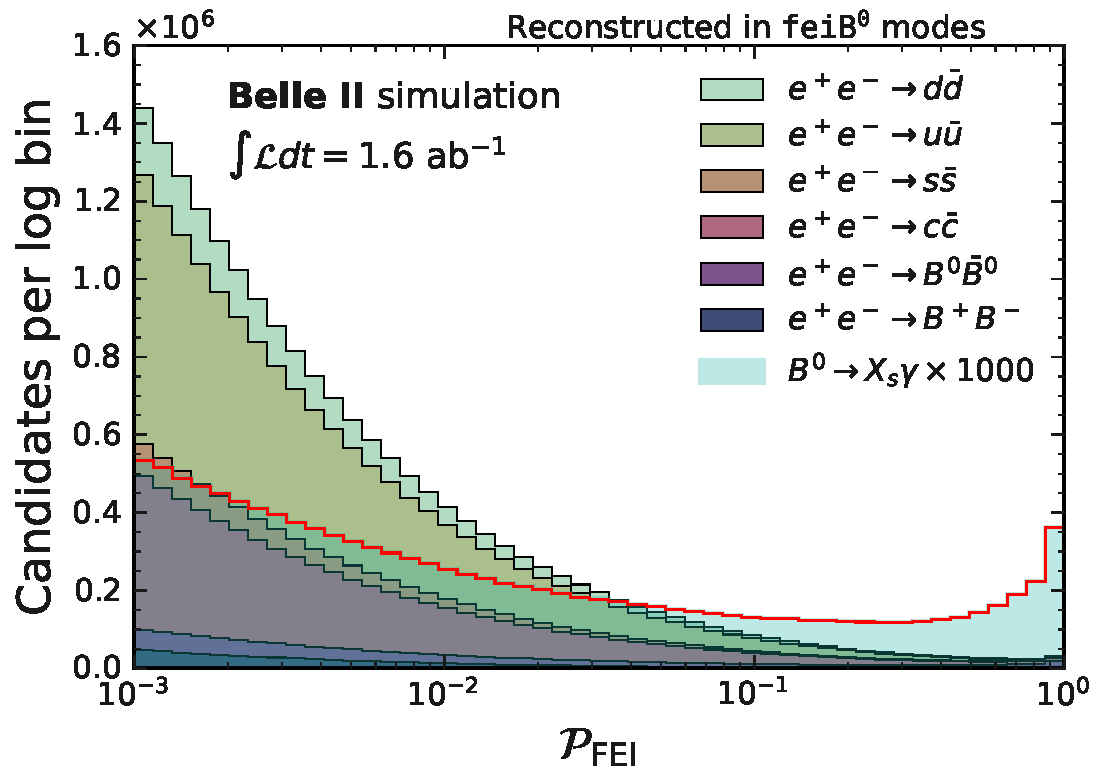
\includegraphics[width=0.45\textwidth]{figures/event_reconstruction/Bz_tagged_background_feiSigProb.pdf}
    }
    \caption{\label{fig:sigprob_after_reco} Tag-side \feiProb after reconstructing \BtoXsgamma events in generic \MC in \feiBp and \feiBz modes.
    Overlaid are events from signal \MC, where the photon comes from \BtoXsgamma, multiplied by a scaling factor.
    These figures may include multiple tag-$B$ and photon entries per event.
    }
\end{figure}

% \subsection{Event topology reconstrunction}
% Many quantities that parametrise the \epem collision product topology in terms of tracks and neutral clusters in the event will be used.
% Using a definition, equivalent to cleaned tracks and clusters we recon